\documentclass[tikz,border=5pt]{standalone}
\usepackage{fontspec}
\setmainfont{Times New Roman}
\usepackage{unicode-math}
\setmathfont{Cambria Math}
\usetikzlibrary{shapes.geometric,positioning,fit,backgrounds,arrows.meta,calc}

\begin{document}
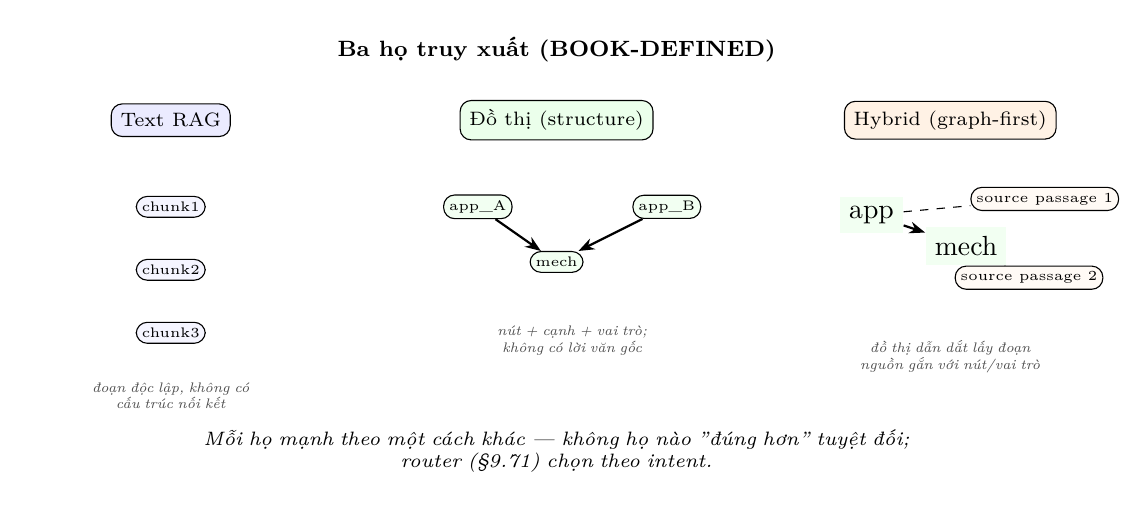
\begin{tikzpicture}[
  unit/.style={rectangle, draw, rounded corners, align=center, font=\tiny, inner sep=2pt},
  box/.style={rectangle, draw, rounded corners, align=center, font=\scriptsize, fill=gray!6},
  arrow/.style={-{Stealth[length=2mm]}, thick},
]

\node[font=\footnotesize\bfseries] at (0, 3.9) {Ba họ truy xuất (BOOK-DEFINED)};

% === Text-only RAG ===
\node[box, fill=blue!8] (t1) at (-4.9, 3.0) {Text RAG};
\node[unit, fill=blue!4] (t2) at (-4.9, 1.9) {chunk1};
\node[unit, fill=blue!4] (t3) at (-4.9, 1.1) {chunk2};
\node[unit, fill=blue!4] (t4) at (-4.9, 0.3) {chunk3};
\node[font=\tiny\itshape, text=gray!60!black, align=center, text width=3.4cm] at (-4.9, -0.5)
  {đoạn độc lập, không có\\cấu trúc nối kết};

% === Graph-only ===
\node[box, fill=green!8] (g1) at (0, 3.0) {Đồ thị (structure)};
\node[unit, fill=green!5] (g2) at (-1.0, 1.9) {app\_A};
\node[unit, fill=green!5] (g3) at (0.0, 1.2) {mech};
\node[unit, fill=green!5] (g4) at (1.4, 1.9) {app\_B};
\draw[thick, -{Stealth[length=2mm]}] (g2) -- (g3);
\draw[thick, -{Stealth[length=2mm]}] (g4) -- (g3);
\node[font=\tiny\itshape, text=gray!60!black, align=center, text width=3.6cm] at (0.2, 0.2)
  {nút + cạnh + vai trò;\\không có lời văn gốc};

% === Hybrid (graph-driven text) ===
\node[box, fill=orange!10] (h1) at (5.0, 3.0) {Hybrid (graph-first)};
\node[fill=green!5] (h2) at (4.0, 1.8) {app};
\node[fill=green!5] (h3) at (5.2, 1.4) {mech};
\draw[thick, -{Stealth[length=2mm]}] (h2) -- (h3);
\node[unit, fill=orange!4] (h4) at (6.2, 2.0) {source passage 1};
\node[unit, fill=orange!4] (h5) at (6.0, 1.0) {source passage 2};
\draw[thin, dashed] (h2) -- (h4);
\draw[thin, dashed] (h3) -- (h5);
\node[font=\tiny\itshape, text=gray!60!black, align=center, text width=3.4cm] at (5.0, 0.0)
  {đồ thị dẫn dắt lấy đoạn\\nguồn gắn với nút/vai trò};

\node[font=\scriptsize\itshape, align=center, text width=12.5cm] at (0, -1.2)
  {Mỗi họ mạnh theo một cách khác — không họ nào "đúng hơn" tuyệt đối;\\router (§9.71) chọn theo intent.};

\end{tikzpicture}
\end{document}